% !TEX root = ../console.tex

\infoTable{双光子纠缠源研究和量子非局域性验证}
{2035年3月7日，周八全天}
{教学楼物理实验室666暗室}
{室温2200摄氏度}
{代码人 12345678}
{\textcolor{StructureColor}{\textbf{实验人2：}} &  \textbf{实验人 87654321} \\
	\textcolor{StructureColor}{\textbf{实验人3：}} &  \textbf{报告人 00000000} \\
	\textcolor{StructureColor}{\textbf{实验人4：}} &  \textbf{牛马人 11111111} \\}
{问问人}

% 预习报告	
\clearpage
\setcounter{section}{0}
\section{预习报告}

\subsection{实验概述}
本实验围绕“\textbf{双光子纠缠源的制备与量子非局域性的验证}”展开，旨在通过偏振纠缠态生成、自发参量下转换的机理探究及\textbf{保真度、对比度、CHSH 游戏胜率}等多重测量手段，全面刻画并检验量子力学的非经典关联。

报告首先回顾了相关量子力学与量子光学基础，包括纠缠态与密度矩阵的表征、电磁场量子化的核心框架以及原子-光场相互作用的简要模型，然后结合实验设计和光学器件调控原理，重点介绍了测试模块的搭建、校准、数据采集与测量基设定等过程。通过对比度及保真度的量化分析，我们\textbf{评估了制备态在偏振自由度上的干涉可见度与理想态一致性}，并以 CHSH 游戏作为非局域性判据，成功观测到实验胜率超过经典极限，从而印证了双光子纠缠态的量子特性。虽然部分测量仍存在角度偏差和装置不稳定等问题，但在报告的分析与讨论中，我们深入探讨了误差来源，并提出了相应的改进策略，从而为后续更高精度的量子态制备和非局域性验证打下基础。

值得一提的是，我们还自行实现并对比了不同\textbf{量子态断层扫描}算法（如线性反演和基于最大似然估计的 iMLE 方法），以进一步揭示数值方法和实验细节之间的耦合关系。

总体而言，这项实验在为我们提供亲身感受量子纠缠与非局域性魅力的同时，也展示了在偏振调控、相干测量与误差修正等方面的综合实力，最后谨\textbf{向给予我们指导与帮助的老师与助教致以诚挚的感谢}。

\subsection{实验原理}

\subsubsection{基本物理学知识的回顾}
\begin{enumerate}
	\item 量子力学核心内容的简要回顾
	
	物理体系的状态由态矢量 \(\ket{\psi}\) 或密度算符 \(\rho\) 表征，处在抽象的希尔伯特空间中。对单个两能级量子比特，其希尔伯特空间可视为二维复向量空间；对于光子偏振态，则相应为以 \(\{\ket{H},\ket{V}\}\) 为基的一组正交态。
	
	量子测量对应厄米算符（可观测量）的本征分解，不同测量基会导致不同的测量结果统计分布。这也是 Bell 测试、CHSH 游戏等检验非局域性的基础原理。
	
	量子系统允许线性叠加态存在，如\(\ket{\psi} = \alpha\ket{H} + \beta\ket{V}\)。两子系统的态叠加亦会引导出纠缠现象，当无法用单个部分的态乘积来描述整体时，就称系统产生了纠缠。
	
	量子系统遵从薛定谔方程（封闭体系）或主方程（开放体系）演化，各种对称性（如幺正对称、守恒量）在具体求解和模型化时发挥重要作用。
	
	在本实验中，最核心的量子力学内容便是：\(\ket{HH} + \ket{VV}\) 类型的纠缠态将导致对测量基的依赖性符合计数分布，以及超越经典理论的量子关联（非局域性）。
	
	\item 纠缠态与密度矩阵
	
	纠缠态是一种复合量子系统中各部分无法用独立态描述的非因果性态。\textbf{两粒子系统的纯态无法分解为子系统的直积态，即存在非经典关联。}例如偏振纠缠态：
	\[
	|\varphi\rangle = \frac{1}{\sqrt{2}}(|HH\rangle + |VV\rangle)
	\]
	测量一粒子会瞬间确定另一粒子状态，即使两者类空分离（量子非局域性）。例如，标准的 Bell 态 \(|\Phi^+\rangle = \frac{1}{\sqrt{2}}(|00\rangle + |11\rangle)\) 满足：对任意局域测量，测量结果之间呈现强相关性，但该相关性不能用局域隐变量理论解释。
	
	密度矩阵 \(\rho\) 是一种对混合态和测量统计自然描述的数学对象，定义为：
	\[ \rho = \sum_i p_i |\psi_i\rangle\langle \psi_i|, \quad \sum_i p_i = 1 \]
	其中 \(|\psi_i\rangle\) 是纯态，\(p_i\) 是其概率。
	
	\textbf{纠缠态的密度矩阵无法分解为任意两个子系统的张量积形式}：
	\[ \rho_{AB} \neq \sum_i p_i \rho_A^{(i)} \otimes \rho_B^{(i)} \]
	其非可分性是量子非局域性的根本来源。
	
	\item 量子光学相关
	
	首先我们考虑\textbf{电磁场的量子化}。经典麦克斯韦场在自由空间中可表示为简谐模的叠加，量子化处理则将每一模视为一组谐振子：
	\[ H = \sum_k \hbar \omega_k \left(a_k^\dagger a_k + \frac{1}{2}\right) \]
	其中 \(a_k, a_k^\dagger\) 为模 \(k\) 的湮灭与产生算符。态空间为所有模的 Fock 空间。
	
	模式展开：
	$$
	\boldsymbol{E}=\sum_j \boldsymbol{E}_j, \quad \boldsymbol{B}=\sum_j \boldsymbol{B}_j, \quad H=\sum_j H_j
	$$
	
	一维驻波：
	$$
	\begin{gathered}
		E_j(z, t)=E_j^{(s)} \sin \left(k_j z\right)\left[a_j \mathrm{e}^{-\mathrm{i}\omega_j t}+a_j^{+} \mathrm{e}^{\mathrm{i} \omega_j t}\right] \\
		B_j(z, t)=-\mathrm{i} B_j^{(s)} \cos \left(k_j z\right)\left[a_j \mathrm{e}^{-\mathrm{i} \omega_j t}-a_j^{+} \mathrm{e}^{\mathrm{i} \omega_j t}\right]
	\end{gathered}
	$$
	或
	$$
	\begin{aligned}
		& E_j=\mathrm{i} E_j^{(0)} \sin \left(k_j z\right)\left[a_j \mathrm{e}^{-\mathrm{i}\omega_j t}-a_j^{+} \mathrm{e}^{\mathrm{i}\omega_j t}\right] \\
		& B_j=B_j^{(0)} \cos \left(k_j z\right)\left[a_j \mathrm{e}^{-\mathrm{i}\omega_j j}+a_j^{+} \mathrm{e}^{\mathrm{\omega}_j t}\right]
	\end{aligned}
	$$
	其中，$E_j^{(s)}=E_j^{(0)}=\sqrt{\hbar \omega_j / V \varepsilon_0} ; B_j^{(s)}=B_j^{(0)}=E_j^{(0)} / c 。$
	
	行波形式
	$$
	\begin{gathered}
		\boldsymbol{E}_j(\boldsymbol{r}, t)=\mathrm{i} \boldsymbol{e}_j E_j^{(r)}\left\{a_j \mathrm{e}^{-\mathrm{i}\left(\omega_k t-\boldsymbol{k}_j \cdot \boldsymbol{r}\right)}-a_j^{+} \mathrm{e}^{\mathrm{i}\left(\omega_k t-\boldsymbol{k}_j \cdot \boldsymbol{r}\right)}\right\} \\
		\boldsymbol{B}_j(\boldsymbol{r}, t)=\mathrm{i}\left(\frac{\boldsymbol{k}_j}{k_j} \times \boldsymbol{e}_j\right) B_j^{(r)}\left\{a_j \mathrm{e}^{-\mathrm{i}\left(\omega_k t-\boldsymbol{k}_j \cdot \boldsymbol{r}\right)}-a_j^{+} \mathrm{e}^{\mathrm{i}\left(\omega_k t-\boldsymbol{k}_j \cdot \boldsymbol{r}\right)}\right\}
	\end{gathered}
	$$
	其中，$E_j^{(r)}=\sqrt{\hbar \omega_j / 2 V \varepsilon_0} ; B_j^{(r)}=E_j^{(r)} / c$ 。
	
	对于量子化电磁场，它有一些典型态。\textbf{Fock态（数态）}：\(|n\rangle\) 是粒子数确定的本征态；\textbf{相干态}：最接近经典光场的态，由激光产生；其为谐振子上的最小不确定态$ a|\alpha\rangle = \alpha|\alpha\rangle $，激光脉冲经强衰减后成为“弱相干态”，但其光子数仍服从泊松分布，因此单光子出现概率低，不能形成真正的单光子源；\textbf{压缩态}：对特定象限的不确定性低于真空态的高斯态，可由非线性晶体实现参量下转换（SPDC）过程产生。
	
	进一步考虑考虑光与原子相互作用，$H = H_0 + V$；其中$H_0 = \sum_{k}\hbar\omega_k\ket{k}\bra{k}$给出自由原子项；考虑可见光波长，相互作用项采取\textbf{偶极矩近似}，即$V = -\vec{d}\cdot\vec{E}$，而$\vec{d} = \sum_{j,k}\vec{d_{j,k}}\ket{j}\bra{k}$。通常在\textbf{相互作用绘景}下对体系演化进行计算。$\ket{\psi_I(t)} = \sum_nc_n(t)\ket{n}$，$i\hbar\dfrac{\partial}{\partial t}\ket{\psi_I(t)} = V_I\ket{\psi_I(t)}$，$V_I = U_0^\dagger V U_0$。
	
	对于半经典理论，在偶极近似相互作用绘景下，光与原子的相互作用可简化为最基本的\textbf{二能级近似}$ H_I = -\vec{\mu} \cdot \vec{E}(t) $，进一步引入\textbf{旋转波近似}（RWA）略去非共振项可导出单模二能级系统吸收/发射过程（如 Rabi 振荡）与双模三能级系统的两光子跃迁行为（级联型、V型和$\Lambda$型）。
	
	对于全量子理论，\textbf{Jaynes-Cummings模型}将光场也视为量子系统，其与二能级原子的耦合形式为：$ H = \hbar \omega a^\dagger a + \frac{1}{2}\hbar \omega_0 \sigma_z + \hbar g (a^\dagger \sigma_- + a \sigma_+) $，该模型展现了真空拉比分裂与共振量子吸收行为。
	
	在实际系统中需考虑环境耦合与退相干过程，\textbf{主方程}提供动力学演化方式：$ \frac{d\rho}{dt} = -\frac{i}{\hbar}[H,\rho] + \mathcal{L}[\rho] $，其中 \(\mathcal{L}[\rho]\) 表示 Lindblad 超算符，用于描述弛豫与退相干。
\end{enumerate}

\subsubsection{自发参量下转换}
在非线性光学中，介质对外加电场的响应并不总是线性的，尤其当电场强度较大时，传统的线性关系
\[
\mathbf{P} = \chi^{(1)} \cdot \mathbf{E}
\]
已无法充分描述实际情况。此时，极化强度 $\mathbf{P}$ 对电场 $\mathbf{E}$ 的响应需要展开为
\[
\mathbf{P} = \chi^{(1)} \cdot \mathbf{E} + \chi^{(2)} : \mathbf{EE} + \chi^{(3)} : \mathbf{EEE} + \cdots
\]
这实际上是对 $\mathbf{P}$ 关于矢量 $\mathbf{E}$ 的泰勒展开，不同于标量函数的泰勒展开，这里每一项均涉及张量形式。介质具有这种非线性响应特性的，即被称为\textbf{非线性介质}。

非线性介质中出现许多有趣的现象，其中之一是\textbf{新频率分量的产生}。为了便于理解这一点，设单色电磁波为
\[
\mathbf{E} = \mathbf{E}_0 e^{-i \omega t} + \text{c.c.}
\]
代入上式可发现由于 $\chi^{(2)}$ 项中涉及 $\mathbf{E}^2$，因此 $\mathbf{P}$ 中将出现频率为 $2\omega$ 的分量，即倍频分量；类似地，由于 $\chi^{(3)}$ 项的存在，还会出现三倍频分量等更高次谐波分量。

上述非线性过程的量子版本可通过如下的电磁场哈密顿量描述：
\[
H_{\text{em}} \approx H_{\text{em}}^{(0)} + H_{\text{em}}^{(3)}
\]
其中
\[
H_{\text{em}}^{(0)} = \sum_{ks} \hbar \omega_{ks} a_{ks}^\dagger a_{ks}
\]
是电磁场的自由哈密顿量，而三阶相互作用哈密顿量为：
\[
H_{\text{em}}^{(3)} = \frac{i}{V^{3/2}} \sum_{\vec{k}_0 s_0} \sum_{\vec{k}_1 s_1} \sum_{\vec{k}_2 s_2} C(\vec{k}_0 - \vec{k}_1 - \vec{k}_2) \, \delta_{\omega_0, \omega_1 + \omega_2} \, g^{(3)}_{s_0 s_1 s_2} \left[ a_{\vec{k}_1}^\dagger a_{\vec{k}_2}^\dagger a_{\vec{k}_0} - \text{H.C.} \right]
\]

考虑实验中由激光泵浦产生的单模光场 $|\alpha\rangle$，当其作用于真空态并经历上述三阶哈密顿量作用时，将诱导\textbf{信号光子（signal）与闲置光子（idler）}的产生，可简表示为：
\[
|\alpha\rangle \otimes |vac\rangle_s \otimes |vac\rangle_i \xrightarrow{H} |\alpha\rangle \otimes |1\rangle_s \otimes |1\rangle_i
\]

在相互作用绘景下，若令 $a_k^{(I)}(t) = a_k^{(S)} e^{-i\omega_k(t - t_0)}$，则哈密顿量演化为：
\[
H_{\text{em}}^{(3)}(t) = -\frac{i}{V} \sum_{\vec{k}_1, \vec{k}_2} G^{(3)} C(\vec{p} - \vec{k}_1 - \vec{k}_2) e^{-i\Delta t} a_{\vec{k}_1}^\dagger a_{\vec{k}_2}^\dagger + \text{H.C.}
\]
其中 $\Delta = \omega_p - \omega_1 - \omega_2$。令初始态为 $|\Psi(t)\rangle = |0\rangle + |\Psi^{(1)}(t)\rangle + \cdots$，利用微扰论可得一阶微扰态：
\[
|\Psi^{(1)}(t)\rangle = -\frac{1}{V} \sum_{\vec{k}_1, \vec{k}_2} \hbar \, C(\vec{p} - \vec{k}_1 - \vec{k}_2) \, e^{-i\Delta t/2} \frac{\sin(\Delta t/2)}{\Delta} a_{\vec{k}_1}^\dagger a_{\vec{k}_2}^\dagger |0\rangle
\]

在体积趋于无穷的极限下，求和转为积分：
\[
|\Psi(t)\rangle = |0\rangle - \int \frac{d^3k_1}{(2\pi)^3} \int \frac{d^3k_2}{(2\pi)^3} \frac{2G^{(3)}}{\hbar} (2\pi)^3 \delta(\vec{p} - \vec{k}_1 - \vec{k}_2) e^{-i\Delta t/2} \frac{\sin(\Delta t/2)}{\Delta} a^\dagger(\vec{k}_1) a^\dagger(\vec{k}_2) |0\rangle
\]
在演化时间 $t \to \infty$ 时，利用极限
\[
\lim_{t \to \infty} e^{-i\Delta t/2} \frac{\sin(\Delta t/2)}{\Delta} = \frac{\pi}{2} \delta(\Delta)
\]
最终得到：
\[
|\Psi(\infty)\rangle = |0\rangle - \int \frac{d^3k_1}{(2\pi)^3} \int \frac{d^3k_2}{(2\pi)^3} \frac{G^{(3)}}{2\hbar} (2\pi)^3 \delta(\vec{p} - \vec{k}_1 - \vec{k}_2) (2\pi) \delta(\omega_p - \omega_1 - \omega_2) a^\dagger(\vec{k}_1) a^\dagger(\vec{k}_2) |0\rangle
\]

这正是一个\textbf{双光子纠缠态}。这一过程被称为\textbf{自发参量下转换（Spontaneous Parametric Down-Conversion, SPDC）}。称其为“自发”，是因为经典非线性光学中若无 signal 光，则 idler 无法单独出现；而量子电磁场的真空涨落可以自发触发整个过程。

在实际应用中，我们关注的不仅是光子对的产生，还希望它们具有可观测的纠缠性质。SPDC 过程中产生的信号光与闲置光具有“频率关联”，即其频率满足 $\omega_s + \omega_i = \omega_p$。为了描述频率关联的细节，引入 $\Phi(k_3; k_1, k_2)$ 表示三者的耦合振幅，其形式为：
\[
\Phi(k_3; k_1, k_2) \propto \delta(\omega_3 - \omega_1 - \omega_2) \, \text{sinc}(\Delta k L)
\]
其中 $\Delta k = k_3 - k_1 - k_2$ 是相位不匹配量，$L$ 是非线性晶体的有效长度。频率关联依赖能量守恒与动量守恒（即 $\Delta k = 0$），同时也决定了光子对产生的效率。

\begin{figure}[h!]
	\centering
	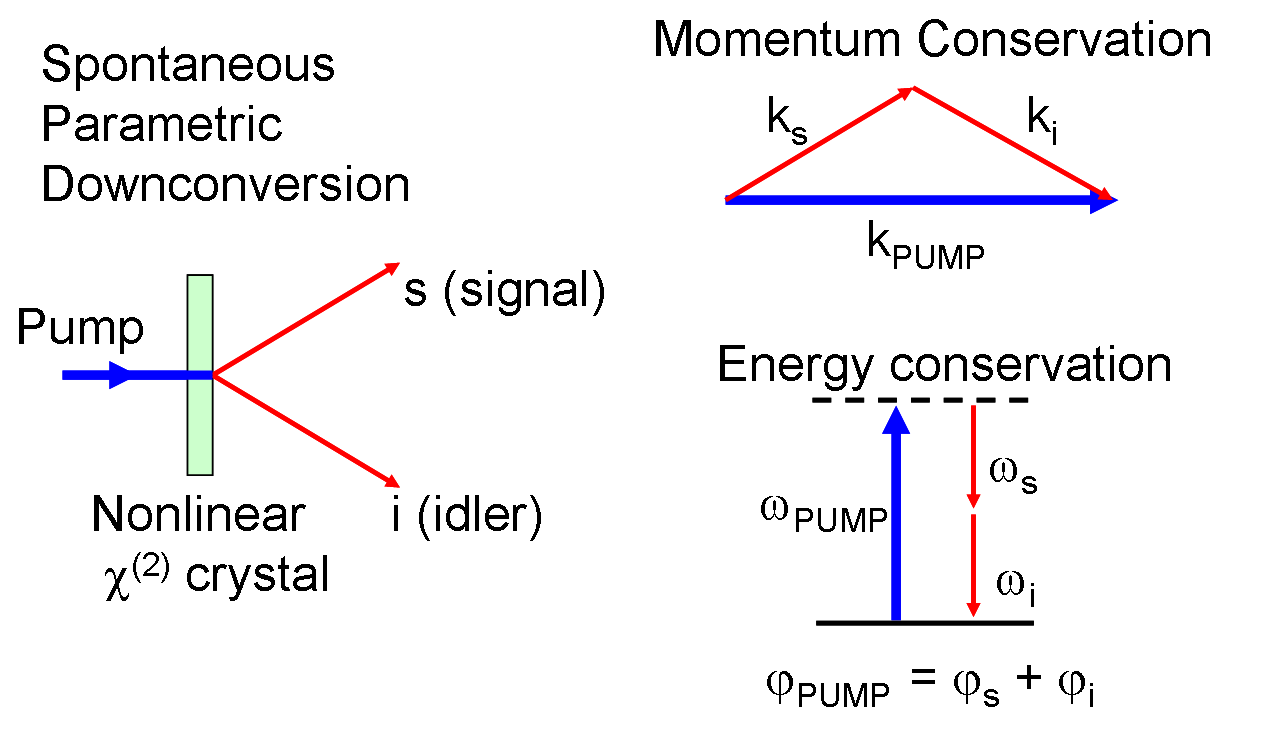
\includegraphics[width=0.7\linewidth]{images/apl2_5_spontaneous_parametric_downconversion}
	\caption{SPDC 过程示意图，守恒定律针对晶体内部的能量和动量（\cref{ref:c}）。}
	\label{fig:apl25spontaneousparametricdownconversion}
\end{figure}

由于信号光与闲置光的频率与动量为连续变量，故频率与动量纠缠虽存在，但难以利用。更常见的是通过\textbf{双折射非线性晶体}的相位匹配结构实现\textbf{偏振纠缠态}。利用晶体的双折射特性，构造出 Type-I 与 Type-II 相位匹配：

\begin{itemize}
	\item \textbf{Type-I}：pump 为 e 光，signal 和 idler 为 o 光，有
	\[
	\Delta k = k_e(\omega_p) - k_o(\omega_s) - k_o(\omega_i) = 0
	\]
	\item \textbf{Type-II}：pump 和 signal 为 o 光，idler 为 e 光，有
	\[
	\Delta k = k_o(\omega_p) - k_o(\omega_s) - k_e(\omega_i, \theta) = 0
	\]
\end{itemize}

由于 e 光与 o 光在偏振方向上不同，因此在满足相位匹配的条件下，SPDC 所产生的信号光与闲置光在偏振上表现出纠缠关系。这种由双折射非线性晶体实现的纠缠通常称为\textbf{偏振纠缠}，其在量子信息处理和基础量子力学研究中具有重要应用价值。

\subsubsection{CHSH 游戏}
\begin{enumerate}
	\item 规则
	
	有两位玩家：爱丽丝（Alice）和鲍勃（Bob）。他们事先可以协商策略（包括共享量子态），但在游戏开始后不能再通信。裁判分别给爱丽丝、鲍勃各一个比特 \( x, y \in \{0,1\} \)（可理解为随机的 00,01,10,11 四种输入各占 1/4 的概率） 。 爱丽丝、鲍勃在各自接收到输入后，须分别输出一个比特 \( a, b \in \{0,1\} \)。
	
	\textbf{胜利条件}为：
	$$ a + b = xy(mod2)   $$
	也就是说，当裁判给出 \((x,y)\)，爱丽丝和鲍勃分别输出 \((a,b)\) 后，如果满足 \(a \oplus b = x y\)，则他们在该局游戏中“赢”，否则“输”。
	
	\item 经典策略
	
	如果允许爱丽丝和鲍勃使用任何经典（含随机性但不含量子纠缠）的策略，容易证明他们最多只能以 75\%（即 3/4）概率赢下此游戏。
	
	对于确定策略：
	\begin{itemize}
		\item \textbf{Strategy: Always Send 0}
		\begin{itemize}
			\item $(x, y) = (0, 0) \Rightarrow (a, b) = (0, 0) \Rightarrow a + b = 0, \; xy = 0$
			\item $(x, y) = (0, 1) \Rightarrow (a, b) = (0, 0) \Rightarrow a + b = 0, \; xy = 0$
			\item $(x, y) = (1, 0) \Rightarrow (a, b) = (0, 0) \Rightarrow a + b = 0, \; xy = 0$
			\item $(x, y) = (1, 1) \Rightarrow (a, b) = (0, 0) \Rightarrow \textcolor{flameorange}{a + b = 0} vs. \textcolor{flameorange}{xy = 1}$
		\end{itemize}
		
		\item \textbf{Strategy: Always Send 1}
		\begin{itemize}
			\item $(x, y) = (0, 0) \Rightarrow (a, b) = (1, 1) \Rightarrow a + b = 0, \; xy = 0$
			\item $(x, y) = (0, 1) \Rightarrow (a, b) = (1, 1) \Rightarrow a + b = 0, \; xy = 0$
			\item $(x, y) = (1, 0) \Rightarrow (a, b) = (1, 1) \Rightarrow a + b = 0, \; xy = 0$
			\item $(x, y) = (1, 1) \Rightarrow (a, b) = (1, 1) \Rightarrow \textcolor{flameorange}{a + b = 0} vs. \textcolor{flameorange}{xy = 1}$
		\end{itemize}
		
		\item \textbf{Strategy: Same as Input}
		\begin{itemize}
			\item $(x, y) = (0, 0) \Rightarrow (a, b) = (0, 0) \Rightarrow a + b = 0, \; xy = 0$
			\item $(x, y) = (0, 1) \Rightarrow (a, b) = (0, 1) \Rightarrow \textcolor{flameorange}{a + b = 1} vs. \textcolor{flameorange}{xy = 0} $
			\item $(x, y) = (1, 0) \Rightarrow (a, b) = (1, 0) \Rightarrow \textcolor{flameorange}{a + b = 1} vs. \textcolor{flameorange}{xy = 0}$
			\item $(x, y) = (1, 1) \Rightarrow (a, b) = (1, 1) \Rightarrow \textcolor{flameorange}{a + b = 0} vs. \textcolor{flameorange}{xy = 1}$
		\end{itemize}
		
		\item \textbf{Strategy: Opposite of Input}
		\begin{itemize}
			\item $(x, y) = (0, 0) \Rightarrow (a, b) = (1, 1) \Rightarrow a + b = 0, \; xy = 0$
			\item $(x, y) = (0, 1) \Rightarrow (a, b) = (1, 0) \Rightarrow \textcolor{flameorange}{a + b = 1} vs. \textcolor{flameorange}{xy = 0}$
			\item $(x, y) = (1, 0) \Rightarrow (a, b) = (0, 1) \Rightarrow \textcolor{flameorange}{a + b = 1} vs. \textcolor{flameorange}{xy = 0}$
			\item $(x, y) = (1, 1) \Rightarrow (a, b) = (0, 0) \Rightarrow \textcolor{flameorange}{a + b = 0} vs. \textcolor{flameorange}{xy = 1}$
		\end{itemize}
	\end{itemize}
	
	\textbf{不确定策略是所有确定策略的凸组合}，因此由上述确定策略即可得经典策略最大胜率为75\%。
	
	\item 量子策略
	
	如果爱丽丝和鲍勃分别持有 Bell pair $\frac{\ket{00} + \ket{11}}{\sqrt{2}}$ 的一个 qubit，则通过以下策略，最大的成功概率是 85\%！
	
	先看两对正交基：
	\begin{enumerate}
		\item 
		\[
		\begin{aligned}
			\ket{\frac{\pi}{8}} &= \cos\left(\frac{\pi}{8}\right)\ket{0} + \sin\left(\frac{\pi}{8}\right)\ket{1}, \\
			\ket{\frac{5\pi}{8}} &= \cos\left(\frac{5\pi}{8}\right)\ket{0} + \sin\left(\frac{5\pi}{8}\right)\ket{1}
		\end{aligned}
		\]
		
		\item 
		\[
		\begin{aligned}
			\ket{-\frac{\pi}{8}} &= \cos\left(-\frac{\pi}{8}\right)\ket{0} + \sin\left(-\frac{\pi}{8}\right)\ket{1}, \\
			\ket{\frac{3\pi}{8}} &= \cos\left(\frac{3\pi}{8}\right)\ket{0} + \sin\left(\frac{3\pi}{8}\right)\ket{1}
		\end{aligned}
		\]
	\end{enumerate}
	
	游戏策略如下：
	\begin{itemize}
		\item $x = 0$: 爱丽丝用 $\{\ket{0}, \ket{1}\}$ 基测量，如果结果为 $\ket{0}$ 则返回 $a = 0$，如果为 $\ket{1}$ 则返回 $a = 1$
		\item $x = 1$: 爱丽丝用 $\{\ket{+}, \ket{-}\}$ 基测量，如果结果为 $\ket{+}$ 则返回 $a = 0$，如果为 $\ket{-}$ 则返回 $a = 1$
		\item $y = 0$: 鲍勃用 $\left\{ \ket{\frac{\pi}{8}}, \ket{\frac{5\pi}{8}} \right\}$ 基测量，如果结果为 $\ket{\frac{\pi}{8}}$ 则返回 $b = 0$，如果为 $\ket{\frac{5\pi}{8}}$ 则返回 $b = 1$
		\item $y = 1$: 鲍勃用 $\left\{ \ket{-\frac{\pi}{8}}, \ket{\frac{3\pi}{8}} \right\}$ 基测量，如果结果为 $\ket{-\frac{\pi}{8}}$ 则返回 $b = 0$，如果为 $\ket{\frac{3\pi}{8}}$ 则返回 $b = 1$
	\end{itemize}
	其最大成功概率为 $\cos^2\left(\frac{\pi}{8}\right) = 85\%$！
	
\end{enumerate}

\subsection{前思考题}
\begin{question}
	在实验内容 2.2 节-测试光路调节中， 为什么第 (4) 步要任意旋转半波片使符合仪计数最大？如果不旋转就去调节符合仪延时和准直器会有什么问题？
\end{question}

旋转半波片的目的是调整光子的偏振方向，使其与符合计数仪的测量基矢匹配，从而最大化符合计数。如果不旋转半波片，仅靠调整符合计数仪的延时和准直器，可能无法优化偏振态匹配，导致符合计数偏低，影响实验数据的准确性和后续分析的精度。因此，这一步是确保光路优化和实验结果可靠性的重要环节。

\begin{question}
	在实验内容 3.1 节-纠缠亮度和对比测量中， +/-基对比度可以表征实验所制备纠缠态$|\varphi \rangle = \frac{1}{\sqrt{2}}(|HH \rangle \pm e^{i \phi}|VV \rangle)$ 的哪一个参数？为什么？
\end{question}

\(+/-\)基对比度可以表征纠缠态 \(|\varphi \rangle = \frac{1}{\sqrt{2}}(|HH \rangle \pm e^{i \phi}|VV \rangle)\) 中的相位参数 \(\phi\)。这是因为在 \(+/-\)基（即 \(|+\rangle = \frac{1}{\sqrt{2}}(|H\rangle + |V\rangle)\) 和 \(|-\rangle = \frac{1}{\sqrt{2}}(|H\rangle - |V\rangle)\)）下进行测量时，符合计数的振荡行为与相位 \(\phi\) 直接相关。通过测量在 \(+/-\)基下的符合计数对比度，可以确定纠缠态的相对相位，从而判断实验制

\begin{question}
	尝试推导并解释 CHSH 游戏中量子世界如何选取最优测量基的方向？
\end{question}

在CHSH游戏中，量子世界可通过选择特定的测量基方向来最大化胜率，从而违背经典极限。

首先应当选用使用最大纠缠态，即贝尔态$|\Phi^+ \rangle = \frac{1}{\sqrt{2}}(|HH \rangle + |VV \rangle)$ 。此态在任意相同测量基下表现出完美关联。

Alice的测量基：当裁判的问题 $x=0$时，选择水平/垂直基（0°）；当$x=1$时，选择对角线基（45°）。对应的量子态投影方向为：
\[
|v_0^A \rangle = |H \rangle , \quad |v_1^A \rangle = \frac{1}{\sqrt{2}} (|H \rangle + |V \rangle)
\]

Bob的测量基：当裁判的问题$y=0$时，选择22.5°方向；当$y=1$时，选择-22.5°方向。对应的投影方向为：
\[
|v_0^B \rangle = \cos(\frac{\pi}{8}) |H \rangle + \sin(\frac{\pi}{8}) |V \rangle , \quad |v_1^B \rangle = \cos(\frac{\pi}{8}) |H \rangle - \sin(\frac{\pi}{8}) |V \rangle
\]

Alice的两个测量基夹角为45°，Bob的两个基夹角为45°，而Alice与Bob的基之间夹角为22.5°。这种对称设计使得量子关联最大化。

通过计算不同测量基组合的期望值$E(x,y)$，CHSH参数$S$可表示为：
\[
S = E(0, 22.5°) + E(0, -22.5°) + E(45°, 22.5°) - E(45°, -22.5°)
\]

可证明，当测量基满足上述角度时， $S = 2\sqrt{2} \pm $2.828，显著超过经典极限。

\begin{question}
	纠缠态制备为$|\varphi \rangle = \frac{1}{\sqrt{2}}(|HH \rangle + e^{i \phi}|VV \rangle)$ 和 $|\varphi \rangle = \frac{1}{\sqrt{2}}(|HH \rangle - e^{i \phi}|VV \rangle)$，对 CHSH 游戏的胜率以及保真度测量会产生什么影响？
\end{question}

\begin{itemize}
	\item \textbf{对胜率的影响}：
	
	如果初始态带有相位$e^{i\phi}$，即：$|\varphi_+ \rangle = \frac{1}{\sqrt{2}} (|HH \rangle + e^{i\phi} |VV \rangle)$
	
	考虑测量后纠缠态的关联函数：$\langle A_x B_y \rangle = \cos(\theta_a - \theta_B + \phi)$
	
	由于相位 $\phi$ 会改变测量结果的相关性，它影响 Bell 期望值：$S(\phi) = 2 \sqrt{2} \cos(\phi)$
	
	因此，胜率变为：$P(\phi) = \frac{1}{2} + \frac{1}{2\sqrt{2}}\cos(\phi)$
	
	\item \textbf{对保真度的影响}：
	
	保真度定义为：$F = |\langle \psi^+ | \varphi \rangle |^2$
	
	存在相位时，有：
	\[
	F_+ = |\langle \psi^+ | \varphi_+ \rangle |^2 = |\frac{1}{\sqrt{2}} (\frac{1}{\sqrt{2}}(|HH\rangle + |VV\rangle) + e^{-i\phi} \frac{1}{\sqrt{2}}(\frac{1}{\sqrt{2}}(|HH\rangle - |VV\rangle))) |^2
	\]
	\[
	\Rightarrow F_+ = \frac{1}{2} |1 + e^{-i\phi} |^2 = \frac{1 + \cos\phi}{2}
	\]
\end{itemize}

\begin{question}
	实验中会有哪些噪声会影响 CHSH 游戏的胜率？如何减小实验中的噪声？
\end{question}

在实验中，影响 CHSH 游戏胜率（即 Bell 违反程度）的噪声主要来源于 量子态制备、测量、环境干扰等因素。这些噪声会降低量子关联，使得实验结果更接近经典极限（75\%），甚至使得 Bell 不等式不再被违反。

\begin{itemize}
	\item \textbf{量子态制备误差}：
	
	CHSH 游戏通常依赖最大 Bell 纠缠态作为资源。实验中，态制备的误差可能导致量子态偏离理想 Bell 态。
	
	可能的误差来源有：由于光学路径不稳定或相干光源的相位漂移，影响测量关联；如果光学元件（波片、PBS 等）存在误差，偏振态可能偏离理想 Bell 态；单光子源效率不完美，导致实验中检测到的光子对数降低，影响统计精度。
	
	可以尝试采用主动相位锁定系统（如压电移相器或锁相环）补偿相位漂移；或者使用高质量的 PBS（偏振分束器）和波片进行偏振控制，在实验前进行系统误差校准（例如利用汤姆森散射测量偏振纯度）。
	
	\item \textbf{量子测量误差}：
	
	CHSH 游戏依赖于对量子比特的正确测量，但实验中的误差可能导致测量基的不完美。
	
	如，波片角度误差会导致投影测量方向偏离预期，使得关联性下降；光子探测器的效率不一致或探测死时间会影响测量统计；温度波动导致波片或 PBS 特性变化，进而影响测量基设置。
	
	可以尝采用高精度步进电机或压电旋转平台控制波片角度，确保测量基准确性；或采用封闭光学系统，降低环境温度变化对测量基的影响。
\end{itemize}

% 报告主体


%---------------------------------------------------------------------
% 实验
\clearpage
\section{实验}

\subsection{测试模块的搭建与校准}

在开展纠缠态特性测试之前，为确保实验精度与重复性，我们首先完成了测试模块的搭建与校准工作。该工作主要包括偏振相关光学器件的光轴校准以及整体光路的搭建与调试。

偏振器件的光轴精确对准对于后续的偏振投影测量至关重要。我们采用标准偏振态光源，逐一校准各偏振片与偏振分束器的光轴方向。该步骤由牛马人与实验人负责完成，具体的校准结果列于\cref{tab1}。

\begin{table}[!ht]
	\centering
	\resizebox{\textwidth}{!}{\begin{tabular}{|c|c|c|c|c|c|c|c|}
			\hline
			测试器件:PP-A & 极值点功率 & 角度（°） & H投射方向 & 测试器件:PP-B & 极值点功率 & 角度（°） & H投射方向 \\ \hline
			入射光功率（mW） & 18.000 & 237 & 59° & 入射光功率（mW） & 18.700 & 89 & 89° \\ \hline
			~ & 0.056 & 330 & ~ & ~ & 0.015 & 182 & ~ \\ \hline
			~ & 18.200 & 59 & ~ & ~ & 18.600 & 272 & ~ \\ \hline
			~ & 0.056 & 149 & ~ & ~ & 0.015 & 0 & ~ \\ \hline
			测试器件:QWP-A & 极值点功率 & 角度（°） & 光轴角度 & 测试器件:PP-B & 极值点功率 & 角度（°） & 光轴角度 \\ \hline
			入射光功率（mW） & 13.320 & 20 & 20° & 入射光功率（mW） & 12.990 & 75 & 344° \\ \hline
			~ & 6.790 & 65 & ~ & ~ & 6.520 & 119 & ~ \\ \hline
			~ & 13.330 & 111 & ~ & ~ & 12.970 & 163 & ~ \\ \hline
			~ & 6.730 & 153 & ~ & ~ & 6.720 & 209 & ~ \\ \hline
		\end{tabular}
	}
	\caption{偏振片和波片角度校准数据}
	\label{tab1}
\end{table}

随后，我们搭建并调试了测试模块的完整光路系统。该过程主要由实验人和牛马人完成，代码人承担部分辅助工作。最终构建完成的测试模块光路如\cref{fig:apl25experimentalopticalpathdiagram}所示，涵盖了信号与闲置光子路径的导引、投影测量器件的布置以及与计数模块的接口连接。

\begin{figure}[h!]
	\centering
	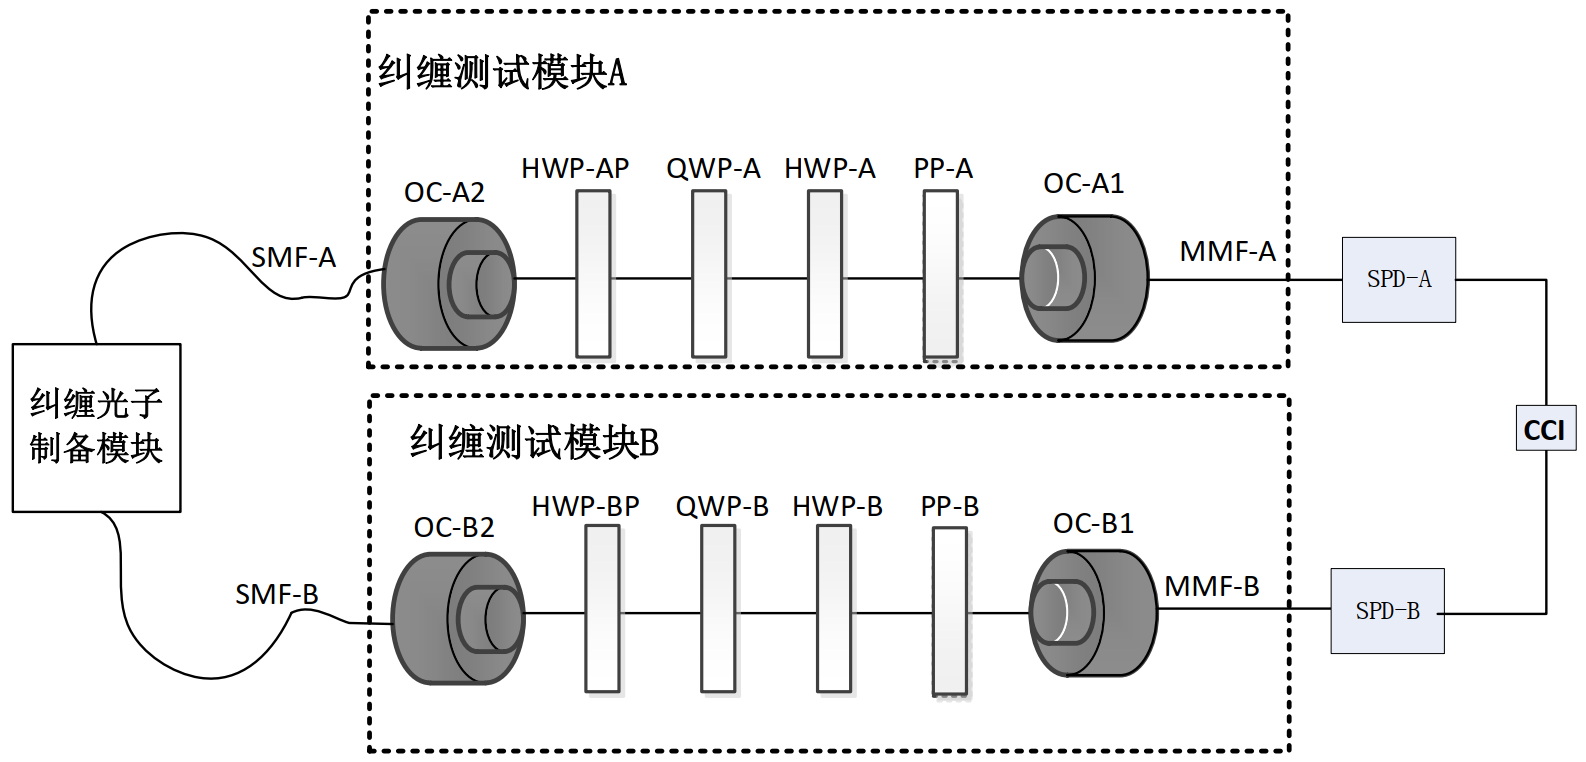
\includegraphics[width=0.9\linewidth]{images/apl2_5_experimental_optical_path_diagram}
	\caption{测试模块的完整光路系统（来自讲义）}
	\label{fig:apl25experimentalopticalpathdiagram}
\end{figure}

至此，实验装置的测试部分已全面搭建完毕，并完成必要的校准工作，为后续的纠缠态验证实验奠定了良好的基础。

\subsection{纠缠特性测试}

我们对纠缠态特性的测试主要包含纠缠亮度和对比度测量、保真度测量以及CHSH 游戏。

\subsubsection{纠缠亮度和对比度测量}
为了评估实验系统产生双光子纠缠态的能力及其质量，我们对纠缠态的亮度和偏振基下的对比度进行了系统测量。实验中使用两个纠缠测试模块，分别标记为 A 和 B。每个模块均配置有一组半波片（HWP-A, HWP-B）与四分之一波片（QWP-A, QWP-B）。具体测量步骤如下：

首先，将 HWP-A 与 HWP-B 均调至 0°，同时将 QWP-A 与 QWP-B 也设定在 0°位置。此时系统处于 $\ket{H}\ket{H}$ 基态的投影设置，记录符合计数仪（Coincidence Counting Instrument, CCI）在积分时间为 10 s 下的符合计数，记为 $C_1$。

随后，将 HWP-A 和 HWP-B 同时旋转至 -45°，对应于 $\ket{V}\ket{V}$ 投影设置，记录符合计数 $C_2$。

接下来，将 HWP-A 从 -45°旋转回 0°，保持 HWP-B 在 -45°，此时对应的符合计数记为 $C_3$。据此可计算单位泵浦光功率下的系统纠缠亮度 $L$，定义为：
\[
L = \frac{C_1 + C_2 - 2C_3}{P}
\]
其中 $P$ 表示入射泵浦光功率。

在对比度测量中，我们首先将 HWP-A 和 HWP-B 同时设定为 -22.5°，对应于 $D/A$ 基的相干投影（即 $\ket{+}\ket{+}$），记录符合计数 $C_4$。随后，将 HWP-A 旋转至 +22.5°，保持 HWP-B 为 -22.5°，记录符合计数 $C_5$。

利用符合计数数据，可分别计算系统在 $H/V$ 基和 $+/-$ 基下的纠缠对比度，定义如下：
\begin{itemize}
	\item $H/V$ 基对比度：
	\[
	V_{HV} = \frac{C_1 - C_3}{C_1 + C_3}
	\]
	
	\item $+/-$ 基对比度：
	\[
	V_{+-} = \frac{C_4 - C_5}{C_4 + C_5}
	\]
\end{itemize}

测量主要由代码人、实验人完成，牛马人记录数据，结果如\cref{tab2}所示。

\begin{table}[h!]
	\centering
	\begin{tabular}{|c|c|c|c|c|c|}
		\hline
		\textbf{通道名称} & \textbf{C1} & \textbf{C2} & \textbf{C3} & \textbf{C4} & \textbf{C5} \\ \hline
		\textbf{通道1} & 29976 & 29210 & 26068 & 28090 & 27499 \\ \hline
		\textbf{通道2} & 13532 & 12700 & 13487 & 13060 & 12539 \\ \hline
		\textbf{OUT} & 1936 & 1376 & 63 & 230 & 1403 \\ \hline
	\end{tabular}
	\caption{纠缠亮度和对比度测量实验数据}
	\label{tab2}
\end{table}

由此计算得到：
$$ V_{HV} = 93.70\% $$
$$ V_{+-} = 71.83 \% $$

$H/V$ 基下的对比度接近理想最大值，表明系统在直线偏振基底中具有良好的干涉可见度，光学器件的校准精度与双光子干涉稳定性较高。与此同时，$+/-$ 基下对比度略低，可能来源于以下因素：光学路径中存在轻微的相位漂移或器件偏差，影响了两个路径之间的相干性；波片的实际相位延迟值与标称值存在偏差，尤其在 $+/-$ 基的干涉测量中更为敏感；计数器或单光子探测器的探测效率非均匀，可能对部分偏振态存在系统性偏倚。

尽管 $+/-$ 基下的对比度相对较低，但其仍明显高于经典系统的典型阈值，说明该实验系统确实制备出了具有非经典相关性的纠缠态。结合两个基底的高对比度表现，可以初步确认所制备态在偏振自由度上具备明显的纠缠特征，为进一步开展量子态层析重构与 Bell 不等式验证实验提供了坚实的基础。

\subsubsection{保真度测量}
为了进一步定量表征实验所制备纠缠态与理想 Bell 态之间的一致性，我们对其进行了保真度测量。该测量基于前述 Bell 不等式测试所用的角度设置，并通过密度矩阵重构获取。

实验过程中，首先根据理论预设的 Bell 不等式测试方案确定各测量基下的半波片旋转角度，并严格按照表格要求调节 HWP-A 与 HWP-B 的偏振角。符合计数数据由符合计数仪（CCI）记录，数据采集工作由代码人与实验人完成，数据记录由牛马人与报告人负责。全部测量结果如\cref{tab3}所示。

\begin{table}[h!]
	\centering
	\begin{tabular}{|l|l|l|l|l|l|}
		\hline
		测量基 & HWP\_A & QWP\_A & HWP\_B & QWP\_B & 符合仪计数 \\ \hline
		HH & 306.00 & 111.00 & 67.00 & 254.00 & 1800 \\ \hline
		HV & 306.00 & 111.00 & 112.00 & 254.00 & 10 \\ \hline
		HL & 306.00 & 111.00 & 89.50 & 254.00 & 800 \\ \hline
		HD & 306.00 & 111.00 & 89.50 & 299.00 & 1050 \\ \hline
		VD & 351.00 & 111.00 & 89.50 & 299.00 & 475 \\ \hline
		VL & 351.00 & 111.00 & 89.50 & 254.00 & 725 \\ \hline
		VH & 351.00 & 111.00 & 67.00 & 254.00 & 15 \\ \hline
		VV & 351.00 & 111.00 & 112.00 & 254.00 & 1150 \\ \hline
		LV & 328.50 & 111.00 & 112.00 & 254.00 & 600 \\ \hline
		LH & 328.50 & 111.00 & 67.00 & 254.00 & 875 \\ \hline
		LL & 328.50 & 111.00 & 89.50 & 254.00 & 100 \\ \hline
		LD & 328.50 & 111.00 & 89.50 & 299.00 & 600 \\ \hline
		DD & 328.50 & 156.00 & 89.50 & 299.00 & 1300 \\ \hline
		DL & 328.50 & 156.00 & 89.50 & 254.00 & 500 \\ \hline
		DH & 328.50 & 156.00 & 67.00 & 254.00 & 750 \\ \hline
		DV & 328.50 & 156.00 & 112.00 & 254.00 & 750 \\ \hline
	\end{tabular}
	\caption{保真度测量实验数据}
	\label{tab3}
\end{table}

随后，采用计算机程序对采集到的符合计数数据进行密度矩阵重构与保真度计算。该部分工作由报告人与实验人协作完成。实验结果如下：

对于理想的 $\ket{\Phi^+} = \frac{1}{\sqrt{2}}(\ket{HH} + \ket{VV})$ 态，即 +Bell 态，计算得两组保真度分别为：
\[
F_1 = 0.9275,\quad F_2 = 0.9151,
\]
平均保真度约为 0.9213 ，表明制备态与目标 Bell 态之间具有较高的一致性，纠缠质量良好。总符合计数为 $E = 2975$。

所重构的密度矩阵如下：

密度矩阵实部：
\[
Re[\rho]=\begin{bmatrix}
	0.5974 & 0.0442 & -0.0538 & 0.4208 \\
	0.0442 & 0.0055 & -0.0037 & 0.0423 \\
	-0.0538 & -0.0037 & 0.0060 & -0.0391 \\
	0.4208 & 0.0423 & -0.0391 & 0.3911 \\
\end{bmatrix}
\]

密度矩阵虚部：
\[
Im[\rho]=\begin{bmatrix}
	0 & -0.0302 & -0.0132 & -0.1303 \\
	0.0302 & 0 & -0.0044 & 0.0128 \\
	0.0132 & 0.0044 & 0 & 0.0244 \\
	0.1303 & -0.0128 & -0.0244 & 0 \\
\end{bmatrix}
\]

同时，我们对其与 -Bell 态 $\ket{\Phi^-} = \frac{1}{\sqrt{2}}(\ket{HH} - \ket{VV})$ 之间的保真度也进行了计算，结果远低，仅为：
\[
F_1 = 0.1065,\quad F_2 = 0.0734,
\]
表明实验所得态与 -Bell 态之间的一致性极低，进一步印证了本次实验系统优先制备的是 $\ket{\Phi^+}$ 态。

事实上，我们对实验室提供的保真度计算程序的计算结果在一定程度上保持怀疑，基于这一原因我们自行探究并尝试开发了用于本实验保真度计算的基于iMLE方法的量子态断层扫描密度矩阵重构方案并得到了不一样的结果，具体内容详见分析与讨论部分。

\subsubsection{CHSH游戏}
为验证实验制备态在量子非局域性测试中的有效性，我们引入 CHSH 游戏框架对系统进行测试。CHSH（Clauser-Horne-Shimony-Holt）游戏是一种量子非局域性验证方式，其核心思想是通过一系列随机选择的局域测量设置，检验系统是否能够超越经典局域隐变量理论所允许的最大胜率上限。

本实验中，采用波片与偏振片组成的偏振基矢选择装置，其中偏振片固定，半波片作为唯一可调元件，用于实现不同测量基的选择。因此，实验的主要操作部件为测试模块中的 HWP-A 与 HWP-B。

由于进行本实验时，我们更换了操作台，新的光学元件标定数据如\cref{tab4}所示。

\begin{table}[h!]
	\centering
	\begin{tabular}{|c|c|c|c|}
		\hline
		\textbf{HWP-A} & \textbf{QWP-A} & \textbf{HWP-B} & \textbf{QWP-B} \\ \hline
		315° & 260° & 226° & 215° \\ \hline
	\end{tabular}
	\caption{CHSH游戏实验台光学元件标定数据}
	\label{tab4}
\end{table}

实验步骤如下：
\begin{enumerate}
	\item 根据 CHSH 游戏的测量方案，构造测量基与输入输出对应关系，并计算 HWP-A 和 HWP-B 所需设置的旋转角度；
	\item 按照数据表格中指定的角度，依次调整两模块中的半波片，并在每一组输入 $(x, y)$ 下记录对应输出 $(a, b)$ 的符合计数值；
	\item 汇总全部测量数据，根据标准 CHSH 游戏胜率定义，计算系统的实际平均胜率。
\end{enumerate}

上述实验操作由报告人与实验人完成，数据统计结果如\cref{tab5}所示。

\begin{table}[h!]
	\centering
	\resizebox{\textwidth}{!}{\begin{tabular}{|c|c|c|c|c|c|c|c|c|}
			\hline
			\textbf{裁判问题} & \textbf{态操作对应的偏振旋转} & \textbf{测量基} & \textbf{HWP-A} & \textbf{} & \textbf{HWP-B} & \textbf{} & \textbf{符合计数} & \textbf{胜率} \\ \hline
			~ & ~ & ~ & 理论值 & 实际值 & 理论值 & 实际值 & ~ & ~ \\ \hline
			X = 0 &  θA0 = 0 & HH & 0 & 315 & 11.25 & 237.25 & 1160 & 77.92\% \\ \hline
			Y = 0 & θB0 = 22.5° & HV & 0 & 315 & -33.75 & 192.25 & 280 & ~ \\ \hline
			~ & ~ & VH & -45 & 270 & 11.25 & 237.25 & 380 & ~ \\ \hline
			~ & ~ & VV & -45 & 270 & -33.75 & 192.25 & 1170 & ~ \\ \hline
			X = 0 &  θA0 = 0 & HH & 0 & 315 & -11.25 & 214.75 & 1180 & 87.21\% \\ \hline
			Y = 1 & θB1 = -22.5° & HV & 0 & 315 & -56.25 & 169.75 & 200 & ~ \\ \hline
			~ & ~ & VH & -45 & 270 & -11.25 & 214.75 & 190 & ~ \\ \hline
			~ & ~ & VV & -45 & 270 & -56.25 & 169.75 & 1480 & ~ \\ \hline
			X = 1 &  θA1 = 45° & HH & 22.5 & 337.5 & 11.25 & 237.25 & 1150 & 76.09\% \\ \hline
			Y = 0 & θB0 = 22.5° & HV & 22.5 & 337.5 & -33.75 & 192.25 & 320 & ~ \\ \hline
			~ & ~ & VH & -22.5 & 292.5 & 11.25 & 237.25 & 390 & ~ \\ \hline
			~ & ~ & VV & -22.5 & 292.5 & -33.75 & 192.25 & 1110 & ~ \\ \hline
			X = 1 &  θA1 = 45° & HH & 22.5 & 337.5 & -11.25 & 214.75 & 470 & 62.82\% \\ \hline
			Y = 1 & θB1 = -22.5° & HV & 22.5 & 337.5 & -56.25 & 169.75 & 1080 & ~ \\ \hline
			~ & ~ & VH & -22.5 & 292.5 & -11.25 & 214.75 & 880 & ~ \\ \hline
			~ & ~ & VV & -22.5 & 292.5 & -56.25 & 169.75 & 690 & ~ \\ \hline
		\end{tabular}
	}
	\caption{CHSH 游戏测量数据}
	\label{tab5}
\end{table}

实验得到的 CHSH 游戏平均胜率为：
\[
P_\text{win} = 76.01\%.
\]

该结果高于经典局域理论所允许的最大胜率 75\%，但偏离理想量子理论上限 $P_\text{win}^\text{quantum} = \cos^2\left(\frac{\pi}{8}\right) \approx 85.36\%$ 较远。实验细节中可能存在的系统误差或相干性损失对结果造成了一定影响，具体讨论详见“分析与讨论”部分。

该测量结果从统计意义上支持了实验所制备纠缠态具备一定的非局域性表现，但同时也反映出实验系统在光学对准、波片误差或计数稳定性等方面仍存在改进空间。

%---------------------------------------------------------------------
% 分析与讨论
\section{分析与讨论}

\subsection{基于iMLE方法的量子态断层扫描与保真度计算}

\subsubsection{保真度}
\textbf{保真度（Fidelity）}是用来衡量两个量子态相似程度的指标，数值范围在 \([0,1]\) 之间，\( F = 1 \) 表示两个量子态完全相同，\( F = 0 \) 表示它们完全不同。

如果两个量子态分别由密度矩阵 \( \rho \) 和 \( \sigma \) 描述，保真度的定义（注意另一种常见的定义为本定义的平方）为：
\[
F(\rho, \sigma) =  \text{Tr} \sqrt{\sqrt{\rho} \sigma \sqrt{\rho}} 
\]
其中，\( \text{Tr} \) 表示矩阵的迹（trace）；\( \sqrt{\rho} \) 表示对密度矩阵 \( \rho \) 取平方根。

对于本实验来说，我们可以认为我们要制备的是Bell态$|\Phi^+\rangle = \frac{1}{\sqrt{2}} (|00\rangle + |11\rangle)$，它的密度矩阵为：
\[
\rho_{\Phi^+} = |\Phi^+\rangle \langle \Phi^+|
\]
\[
= \frac{1}{2} (|00\rangle + |11\rangle)(\langle 00| + \langle 11|)
\]
\[
= \frac{1}{2} \begin{bmatrix} 
	1 & 0 & 0 & 1 \\ 
	0 & 0 & 0 & 0 \\ 
	0 & 0 & 0 & 0 \\ 
	1 & 0 & 0 & 1
\end{bmatrix}
\]

因此我们需要从测量结果中获得我们制备的态的$\rho$，这就要用到量子态断层扫描。

\subsubsection{量子态断层扫描}
\textbf{量子态断层扫描（Quantum State Tomography, QST）}是一种实验技术，用于重构未知的量子态，即测量和推断密度矩阵 \( \rho \) 的方法。在量子信息处理中，QST 是一个重要的工具，广泛用于量子计算、量子通信和纠缠态的实验研究。由于量子测量通常会破坏态本身，并且单次测量只能提供有限的信息，因此无法直接读取量子态，而需要通过一系列不同的测量来重构整个密度矩阵 \( \rho \)。一个 \( d \) 维的量子态（即 \( n = \log_2 d \) 量子比特）可以用 \( d^2 - 1 \) 个独立的参数表示，因此 QST 需要足够多的独立测量来确定这些参数。  

QST 主要依赖于选取合适的测量基进行实验测量，并利用这些测量数据重构密度矩阵。常见的测量基包括泡利算符基（Pauli Basis），即测量泡利矩阵 \( \sigma_x, \sigma_y, \sigma_z \) 的期望值：  
\[
\sigma_x = \begin{bmatrix} 0 & 1 \\ 1 & 0 \end{bmatrix}, \quad
\sigma_y = \begin{bmatrix} 0 & -i \\ i & 0 \end{bmatrix}, \quad
\sigma_z = \begin{bmatrix} 1 & 0 \\ 0 & -1 \end{bmatrix}
\]  
此外，也可以使用 SIC-POVM（对称、信息完整的正定测量）等超完备测量方法以减少统计误差并提高重构精度。在泡利基下，密度矩阵可以表示为  
\[
\rho = \frac{1}{2^n} \sum_{i_1, i_2, ..., i_n} c_{i_1 i_2 ... i_n} \, \sigma_{i_1} \otimes \sigma_{i_2} \otimes ... \otimes \sigma_{i_n}
\]  
其中，\( c_{i_1 i_2 ... i_n} \) 是泡利矩阵的期望值，由实验测量得到：  
\[
c_{i_1 i_2 ... i_n} = \text{Tr}(\rho \cdot (\sigma_{i_1} \otimes \sigma_{i_2} \otimes ... \otimes \sigma_{i_n}))
\]  
通过这些测量结果，我们可以完全重构密度矩阵。  

QST 的实验过程通常包括以下几个步骤：首先制备未知的量子态 \( \rho \)，然后选择一组测量基（如泡利算符基），接着进行大量次测量，每次对量子态进行投影测量，并统计测量结果的频率，最后通过最大似然估计（Maximum Likelihood Estimation, MLE）或贝叶斯估计（Bayesian Estimation）重构密度矩阵。例如，对于单量子比特的情况，其密度矩阵可以表示为  
\[
\rho = \frac{1}{2} (I + a_x \sigma_x + a_y \sigma_y + a_z \sigma_z)
\]  
其中，\( a_x, a_y, a_z \) 是泡利矩阵的期望值：  
\[
a_x = \text{Tr}(\rho \sigma_x), \quad a_y = \text{Tr}(\rho \sigma_y), \quad a_z = \text{Tr}(\rho \sigma_z)
\]  
通过实验测量这些期望值后，即可求得密度矩阵。  

\subsubsection{iMLE方法、结果与后续展望}
为进一步全面表征双光子纠缠态的密度矩阵结构，本实验基于最大似然估计（Maximum Likelihood Estimation, MLE）方法进行量子态断层扫描（Quantum State Tomography）。其中，\textbf{初始密度矩阵采用线性反演（linear inversion）方式获得}，并作为 iMLE 算法的初始输入，最终得到满足物理约束（Hermiticity、正定性与归一性）的密度矩阵。

\begin{itemize}
	\item 实验中采用 $\{H, V, D, L\}$ 四组偏振态作为单比特测量基，其中，$H = \ket{0}$，$V = \ket{1}$，$D = \frac{1}{\sqrt{2}}(\ket{0} + \ket{1})$以及$L = \frac{1}{\sqrt{2}}(\ket{0} + i\ket{1})$。
	
	构造出的 16 个双比特投影测量算符 $\{P_{AB} = \ket{A}\bra{A} \otimes \ket{B}\bra{B}\}$，覆盖了 $HH, HV, \dots, DV$ 全部基对，分别对应一组符合计数实验数据，详见测量统计：
	\[
	\text{总符合计数} = 2975，\quad \text{归一化后用于断层重构的概率矢量 } \{p_i\}
	\]
	
	通过构造线性方程组 $p_i = \operatorname{Tr}(P_i \rho)$ 并利用 Moore–Penrose 伪逆求解得到初始密度矩阵 $\rho_{\text{linear}}$。该矩阵随后进行物理性修正（Hermiticity、谱截断与归一化），以满足基本的量子态约束。最终重构密度矩阵为：
	\[
	\rho_{\text{linear}} =
	\begin{bmatrix}
		0.577 & 0.041 & -0.076 & 0.434 \\
		0.041 & 0.006 & 0.001 & 0.025 \\
		-0.076 & 0.001 & 0.021 & -0.068 \\
		0.434 & 0.025 & -0.068 & 0.396 \\
	\end{bmatrix}
	\]
	
	与理想 Bell 态 $\ket{\Phi^+} = \frac{1}{\sqrt{2}}(\ket{HH} + \ket{VV})$ 的保真度为：
	\[
	F_{\text{linear}} = 0.9592
	\]
	显示出非常接近目标态的纠缠特性。
	
	具体而言，我们首先以 np.outer 构造 $\ket{A}\bra{A} \otimes \ket{B}\bra{B}$ 的双比特测量投影算符，并整理为列表 measurement\_ops。每个测量基对应的实验归一化频率则整理为 measured\_probs。利用这些信息，我们建立了如下形式的线性方程组：
	\[
	\mathbf{p} = A \cdot \text{vec}(\rho),
	\]
	其中 $A$ 是由测量算符 $\{M_i\}$ 的转置张量积构成的矩阵，$\text{vec}(\rho)$ 是将密度矩阵按行展平后的向量。通过 np.linalg.pinv 实现广义逆矩阵求解，得到线性反演的 $\rho_{\text{linear}}$。
	
	\item 进一步采用\textbf{迭代最大似然估计算法（iMLE）}对密度矩阵进行优化重构，具体迭代过程参考文献 \cref{ref:2}所提出的框架。简言之，在线性反演的基础上，我们进一步实现了经典的迭代最大似然估计算法（iMLE），其核心过程是反复构造权重矩阵 $Q$ 并迭代更新 $\rho$，代码结构参考文献 [2] 中提出的方案。实现中我们加入了以下数值优化策略：为避免除以零，对理论概率 $p_i$ 设置下限；保证每一步结果满足 Hermiticity 与正定性（通过特征值截断）；使用 np.linalg.eigh 实现谱分解与重构。最后，通过 QuTiP 提供的 fidelity() 函数，我们分别计算了 $\rho_{\text{linear}}$ 与 $\rho_{\text{MLE}}$ 相对于理想 Bell 态的保真度。
	
	最终获得的密度矩阵为：
	\[
	\rho_{\text{MLE}} =
	\begin{bmatrix}
		0.433 & 0.210 - 0.139i & 0.192 - 0.131i & 0.130 - 0.334i \\
		0.210 + 0.139i & 0.146 & 0.135 - 0.002i & 0.170 - 0.120i \\
		0.192 + 0.131i & 0.135 + 0.002i & 0.125 & 0.159 - 0.109i \\
		0.130 + 0.334i & 0.170 + 0.120i & 0.159 + 0.109i & 0.296 \\
	\end{bmatrix}
	\]
	
	计算其与目标 Bell 态的保真度得：
	\[
	F_{\text{MLE}} = 0.7030
	\]
	
	这一结果低于线性反演所得保真度，也\textbf{显著低于实验室程序计算}所得 $F \approx 0.9213$。这表明在本实验数据及选择的测量基下，\textbf{iMLE 方法的收敛质量较差}，可能由于：投影测量设置未能充分涵盖高灵敏方向（参见 \cref{ref:5}）；观测概率分布中存在统计波动，影响 MLE 收敛；本实验中所用 iMLE 算法迭代方式为最基础型，未做稀释（dilution）或超加速（superfast）优化。
	
	\item 针对当前 iMLE 收敛性不足的问题，可考虑采用以下方法进一步优化密度矩阵重构结果：引入稀释 MLE（diluted MLE）算法 \cref{ref:3}，提升稳定性；使用 \textbf{Superfast MLE 算法} \cref{ref:4}，加速收敛并避免陷入局部最优；利用\textbf{神经网络生成对抗网络（CGAN）方法} \cref{ref:5}，实现数据驱动的稳健态重构。
	
	此外，在文献 \cref{ref:5} 提供的 GitHub 实例中展示了：即使在无噪声的模拟数据下，iMLE 方法仍可能失败，而神经网络方法则成功恢复目标态。这表明数据与测量基的选择对 iMLE 的性能具有高度敏感性。
\end{itemize}

\subsection{CHSH 游戏结果分析}

\subsubsection{对测试模块光学元件作用的探讨}
根据测试模块光路\cref{fig:apl25experimentalopticalpathdiagram}，我们以一路为例子，具体探讨光学元件HWP-AP、QWP-A、HWP-A、PP-A的作用。
\begin{itemize}
	\item \textbf{HWP-AP：通道偏振补偿波片}
	
	HWP-AP 是一块固定角度的半波片，通常用于补偿光纤耦合和自由空间耦合过程引入的偏振旋转或相位延迟。由于光纤具有一定双折射性，输出偏振态可能偏离期望的 $H/V$ 基，HWP-AP 的主要任务是将光子偏振重新调整至标准线性基底，使后续的波片操作具有良好的基准态。
	
	在数学上，半波片对于偏振态 $\ket{\psi}$ 的作用可以表示为：
	\[
	U_{\text{HWP}}(\theta) = \cos(2\theta) \sigma_x + \sin(2\theta) \sigma_y,
	\]
	其中 $\theta$ 为波片光轴相对于水平轴的夹角，$\sigma_x$ 和 $\sigma_y$ 是 Pauli 矩阵。
	
	HWP-AP 通常固定设置为 0° 或 -22.5°，以实现特定基态的标准化。
	
	\item \textbf{QWP-A：圆偏振到线偏振的转换器}
	
	QWP-A 是测试模块中用于引入圆偏振基（$L/R$）信息的关键元件。在量子态断层扫描中，为实现对不同基下的投影测量，必须引入非线性偏振方向（如 $\ket{L} = \frac{1}{\sqrt{2}}(\ket{H} + i\ket{V})$），四分之一波片的作用正是提供该自由度。
	
	QWP 的 Jones 矩阵如下：
	\[
	U_{\text{QWP}}(\theta) = \begin{bmatrix}
		\cos^2\theta + i\sin^2\theta & (1 - i)\cos\theta\sin\theta \\
		(1 - i)\cos\theta\sin\theta & \sin^2\theta + i\cos^2\theta
	\end{bmatrix}.
	\]
	
	QWP-A 可将 $\ket{L}$ 转换为 $\ket{H}$ 或 $\ket{V}$，使系统仍可使用固定偏振片实现圆偏振投影测量。通过旋转 QWP-A 与后续 HWP-A 的角度组合，可以实现对 $H/V$、$D/A$、$L/R$ 三组正交基的全面投影。
	
	\item \textbf{HWP-A：主控投影角设定器}
	
	HWP-A 是本实验测试模块中最核心的控制元件，其旋转角直接决定测量基的选择。通过设定特定角度（如 0°、22.5°、-22.5°、45° 等），可以实现：
	\begin{itemize}
		\item 在 $H/V$ 基下：测量 $\ket{H}$ 或 $\ket{V}$；
		\item 在 $D/A$ 基下：测量 $\ket{+} = \frac{1}{\sqrt{2}}(\ket{H} + \ket{V})$ 或 $\ket{-}$；
		\item 在 $L/R$ 基下：配合 QWP 实现 $\ket{L}$、$\ket{R}$ 投影。
	\end{itemize}
	在 CHSH 游戏和 Bell 不等式测试中，HWP-A 的具体旋转角构成了不同测量设置 $A_0, A_1$，是非局域性验证的关键操作量。
	
	\item \textbf{PP-A（Polarizer）：偏振投影器}
	
	PP-A 是固定的偏振片，设置为 $H$ 或 $V$ 的透射方向。在实验中，其作用是将前面一系列波片调控后的偏振态进行最终投影选择，相当于执行 $\ket{H}\bra{H}$ 或 $\ket{V}\bra{V}$ 的物理测量。
	
	由于偏振片本身无法调节，因此实验中所有的测量基变换都由前置的 HWP/QWP 系统完成，偏振片作为统一终端执行。
	
\end{itemize}

\subsubsection{对实验结果的探讨与分析}
\begin{itemize}
	\item 从原理上回顾，CHSH 游戏中，Alice 和 Bob 接收二进制输入 $x, y \in \{0, 1\}$，输出 $a, b \in \{0,1\}$，若满足：
	\[
	a \oplus b = x \cdot y,
	\]
	则称为“赢得”该轮游戏。
	
	对于制备在理想的 Bell 态 $\ket{\Phi^+} = \frac{1}{\sqrt{2}}(\ket{HH} + \ket{VV})$ 上的系统，若选择测量角度为：
	- $A_0 = 0^\circ,\quad A_1 = 45^\circ$
	- $B_0 = 22.5^\circ,\quad B_1 = -22.5^\circ$
	
	则理论预测的最大胜率为：
	\[
	P_{\text{win}}^{\text{quantum}} = \frac{2 + \sqrt{2}}{4} \approx 85.36\%.
	\]
	
	测量对应的偏振投影方向为：
	\[
	\begin{aligned}
		A_0 &\rightarrow \ket{0},\quad A_1 \rightarrow \frac{\ket{0} + \ket{1}}{\sqrt{2}} \\
		B_0 &\rightarrow \frac{\ket{0} + \ket{1}}{\sqrt{2}},\quad B_1 \rightarrow \frac{\ket{0} - \ket{1}}{\sqrt{2}} \\
	\end{aligned}
	\]
	
	上述映射通过调整 HWP 的角度 $\theta$ 实现投影到 $\cos(2\theta)\ket{H} + \sin(2\theta)\ket{V}$ 上。
	
	从\cref{tab5}可见，HWP-A 与 HWP-B 的实际角度偏离理论角度显著（最大达 $\sim$ 56°），例如理应设置 $-33.75^\circ$ 的 HWP-B 实际角度为 $192.25^\circ$。由于半波片的转换规则为旋转 $2\theta$，这种偏差导致投影态与理论基向量的夹角产生非线性误差，测量基之间的干涉条纹对比度下降，直接影响各投影下的符合概率。
	
	例如，在 $(x,y)=(1,1)$ 的任务中，HH 项计数为 470，远低于其它输入下的 HH 项，这也正是其胜率最低的原因。理论上，该任务对应的赢取概率应与其它输入相近（约 85\%），但由于该配置对应的投影角偏差最大（超过 20°），结果导致量子关联无法有效展示。
	
	以 $(x,y) = (1,1)$ 为例，其四个输出 $(a,b)$ 对应计数如下：$(a,b)=(0,0)$：HH = 470 → 这是“失败”输出；其余为“成功”输出（HV, VH, VV）总计 = 1080 + 880 + 690 = 2650。
	
	胜率计算：
	\[
	P_{\text{win}}^{(x=1,y=1)} = \frac{2650}{3120} = 0.8487 \quad (\text{理应为失败，结果接近理论胜率})
	\]
	但此处反而HH 被认为是成功输出（$a \oplus b = 1$），说明实验记录中可能存在输出标记顺序或判断逻辑与理论定义不一致之处，需要进一步核对编码与测量对应关系。
	
	从整体上看，每组输入 $(x,y)$ 的符合计数在“赢”与“输”之间的比例，与其对应测量基之间的重叠度成正相关，而这又依赖于波片角度设定的准确性。
	
	\item 尽管我们在多个实验环节均观察到了纠缠态的非经典特性，例如 $H/V$ 基对比度达到 93.70\%、保真度线性重构接近 96\%、CHSH 游戏胜率略高于经典上限，但整体实验表现仍与理想量子预测之间存在明显差距，尤其是 CHSH 游戏中仅为 76.01\% 的平均胜率，提示我们对系统性能进行更深层次的反思。
	
	在 CHSH 游戏的四种输入 $(x, y)$ 组合中，某些子任务（如 $(x, y) = (1, 1)$）的胜率仅为 62.82\%，远低于量子理论上限 85.36\%。对具体计数数据分析可知，HWP-A 与 HWP-B 的实际角度设置与理论值间普遍存在数十度偏差，这一问题贯穿多个测试任务，不仅出现在 CHSH 测试，也反复出现在对比度测量和态重构中。
	
	结合实验现象，我们认为系统性误差主要来源于以下几个紧密关联的层面：
	
	首先，实验中所有偏振基的设定均依赖于手动旋转波片角度，而多组波片（特别是 HWP-B）存在明显的角度零点偏移与刻度误差。即便在表面校准后，部分波片仍表现出不稳定性，调节过程中回程偏差大，导致理想投影态的实现存在系统性失真。这一问题在需要多组角度精确组合的 CHSH 游戏和 iMLE 断层扫描中影响尤为显著。
	
	其次，虽然线性反演密度矩阵给出了较高保真度（95.92\%），但迭代最大似然估计（iMLE）重构仅得到 70.30\% 的保真度，暴露出系统在非线性拟合收敛过程中的不稳定性。这与我们在 CHSH 胜率偏低时观察到的状态质量下降趋势相互印证。我们怀疑其中一部分原因是实验状态在不同基投影下表现出强烈的非对称性，即不同投影角度对应的干涉质量差异显著，暗示系统可能未能在所有测量方向上保持稳定的相干性。
	
	此外，我们在调试实验光路过程中遇到了多次光纤耦合效率剧烈变化、单光子探测器响应漂移等问题。实验设备老化、接口不稳、光轴调节灵敏度低等因素叠加，使得整个系统难以实现精确、稳定、可重复的调节。这些技术性困难虽在操作中被不断修正，但仍在测量数据中留下了痕迹。最明显的例子是，+Bell 态保真度可以接近理想，但对 -Bell 态的拟合几乎完全失败（保真度仅 0.07～0.10），表明系统具有一定的偏向性，未能对称地支持所有 Bell 态。
	
	综上所述，CHSH 游戏中的胜率下降并非孤立现象，而是整个实验系统稳定性和控制精度有限的集中体现。波片角度误差、设备调节滞后、态制备不稳定性以及光路对称性不足，交织构成了限制实验精度的主要瓶颈。
\end{itemize}

